%!TEX root = ../username.tex
\chapter[J.S. Bach and \textit{The Well-Tempered Clavier, Book I} BWV 847]{Johann Sebastian Bach – \textit{The Well-Tempered Clavier, Book I Prelude and Fugue in C Minor}, BWV 847 (1722 and 1740)}
 
 Johann Sebastian (J.S.) Bach (1685-1750) is a composer of the Baroque period, which is commonly approximated to be from about 1600 to 1750. He was born on March 31, 1685, in Leipzig, Germany, and is celebrated as the creator of influential works that include \textit{The Well-Tempered Clavier}, \textit{St. Matthew's Passion}, and \textit{Mass in B Minor}. His works are identified by their number in Wolfgang Schmeider's catalog, as Bach-Werke-Verzeichnis (BWV, or in English, \say{Bach's work catalog}). This catalog was first published in 1950, and groups compositions by genre. Das wohltemperierte Clavier (published as two books, the first in 1722 and the second in 1740) is one of Bach's best-known keyboard works. It is translated to English as \textit{The Well-Tempered Clavier}, and is commonly referred to as WTC \autocite{Lindley_2001}.
 
The two books in WTC consist of 24 prelude and fugue pairs, in alternative major and minor keys. The pairs start in C Major, and are arranged in a rising chromatic pattern, ending in B Minor. The first prelude and fugue pair is in C Major, the second pair is in C Minor, the third in C\musSharp{} Major, and so on until the last pair reaches B Minor. WTC was composed to demonstrate the possibilities of playing in every key in an equal-, or near-equal temperament, which was a new concept. 

Temperament is the name given to various tuning methods, in which consonant intervals, mainly the third and the fifth interval, are made to be more or less imperfect, which is to say they are made to be sharper or flatter than they are originally intended \autocite{Grove_1895}. The phrase \say{well-tempered} refers to the use of a tuning system which works equally well in all keys. An octave is divided into 12 semitones of exactly equal intervals \autocite{Whitcomb_2017}. With the use of equal-temperament, every key is equally useable, so the possibilities for musical organization allowed by this functional tonality\footnote{Functional tonality is defined as organizing chords based on their function, i.e., whether a chord is the tonic, predominant, or dominant chord.} is higher \autocite{Marshall_Emery_2019}. This system was opposite to the system more widely used in Bach's time: meantone temperament. Meantone temperament is characterized by the accidentals in a piece's key, and a key with many accidentals sounding out of tune \autocite{Grove_1895}. 

WTC is a combination of several popular musical forms, styles, and genres of Bach's time. These range from popular dance types such as arias\footnote{This is a dance defined as a solo song with an instrumental accompaniment.}\autocite{Marshall_Emery_2019}, motets\footnote{This is defined as a style of vocal composition for one or more soloists and an instrumental accompaniment. It may or may not include a choir.}\autocite{Marshall_Emery_2019}, and concerti. These forms, styles, and genres are then presented within the unified compositional technique: the fugue. A fugue is characterized by the systematic imitation of a main theme, known as the subject, and simultaneously sounding melodic lines, known as the countersubject, which produces counterpoint. \autocite{Marshall_Emery_2019}\footnote{Counterpoint is a term used to describe the combination of simultaneously sounding musical lines, according to a system of rule.}\autocite{Sachs_Dahlhaus_2001} The fugue's subject is normally introduced in the piece's opening bar (or measure) in one of the fugue's three or four voices. If written in three voices, the fugue's subject could be introduced in either the soprano voice (the top voice), the alto voice (the middle voice), or the bass voice (the lowest voice). If the fugue is written in four voices, we add a tenor voice (the second from the lowest voice), forming a SATB voice formation (soprano, alto, tenor, bass, in short). This subject is then restated in a second voice, while the first voice continues with a countersubject. The remaining voices, which have yet to be introduced, are treated similarly, establishing a contrapuntal system. This system will continue for the duration of the fugue.

\section{Prelude in C Minor}

A prelude is a piece based on improvisation, which examines a particular figuration, texture, melodic motif\autocite{Drabkin_2001}\footnote{This can be defined as a short musical idea, which could be melodic, harmonic, rhythmic, or any combination of the three. The motif may be of any size, and is commonly regarded to be the shortest subdivision of a theme or phrase which maintains its identity as an idea.}, rhythmic idea, or a combination of these, in a continuously unfolding manner. Bach's \textit{Prelude in C Minor} follows this convention, as it is a dramatic, yet mechanical, piece. Tempo and articulation are the primary interpretative tools available to the performer, and thus is one of the few pieces written by Bach which contains tempo indications. Simple chordal functions and plain thematic development highlight the importance of tempo and articulation. The various tempo markings, as seen in Figure \ref{fig:prelude-tempo-markings}\autocite{Henle_2009} must be clearly distinct and contrasted by the performer. This is especially important in the adagio and allegro sections, as in Figure \ref{fig:prelude-recitative}\autocite{Henle_2009},
as they form the piece's recitative.\footnote{A recitative can be defined as a type of vocal composition, notably for a single voice, which has the intent of mimicking dramatic speech in song. In reality, its nature varies by era, nationality, origin, and context.}\autocite{Monson_Westrup_Budden_2001} The performer must allow the recitative to have a greater sense of expression and movement than a section such as the presto may allow. The presto section is a fast section, with a series of quickly moving sixteenth notes, as seen in fig \ref{fig:prelude-tempo-markings}\autocite{Henle_2009}. This speed makes an expressive presto section hard to achieve, so the performer instead must allow the section after, the section in Figure \ref{fig:prelude-recitative}\autocite{Henle_2009}, to be musically varied. 
\begin{figure}
    \centering
    \includegraphics[width=0.75\textwidth]{figures/prelude-tempo-markings.jpg}
    \caption{Tempo markings, as seen in Bach's \textit{Prelude in C Minor}}
    \label{fig:prelude-tempo-markings}
\end{figure}

\begin{figure}
    \centering
    \includegraphics[width=0.5\textwidth]{figures/bach-prelude-adagio-allegro.jpg}
    \caption{The recitative as seen in Bach's \textit{Prelude in C Minor}}
    \label{fig:prelude-recitative}
\end{figure}

\begin{figure}
    \centering
    \includegraphics[width=0.5\textwidth]{figures/bach-prelude-motive-one.jpg}
    \caption{The first of several motives found in Bach's \textit{Prelude in C Minor}}
    \label{fig:bach-first-motive}
\end{figure}

The \textit{Prelude in C Minor} contains several important motifs, or motives. The first is the running eighth notes, as seen in the first four bars of the prelude, and in Figure \ref{fig:bach-first-motive}\autocite{Henle_2009}. A second motif is introduced in the coda, at the start of the adagio section, in bars 34-35 of Figure \ref{fig:prelude-recitative}\autocite{Henle_2009}.It is marked by a change in both the piece's texture and tempo. An arpeggiated chord is followed by a rapid succession of thirty-second note.\footnote{This is defined sounding of a chord's notes individually, such that they are sounded in succession, rather than simultaneously. Read more in \cite{Arpeggio_2001}} This new motif is repeated twice, after a succession of sixteenth notes ends the prelude on a Picardy third.\footnote{A Picardy third, as defined in Lantham, \textit{tierce de Picardie}, involves the usage of a major triad chord within a composition that is otherwise in a minor key.}

\subsection{Fast and Furious}

As a piece based in on improvisation, the \textit{Prelude in C Minor} contains only two interpretive tools which I am able to use: tempo and articulation. Tempo markings are clearly notated by Bach, like those in Figure \ref{fig:prelude-tempo-markings}\autocite{Henle_2009}, and thus I must be sure that the contrast between sections is clear to the listener. The \textit{presto} section, which begins in bar 28, increases in speed as both the right-hand and left-hand play fast sixteenth notes. Then, in measure 34, the tempo marking changes to \textit{adagio}, and the speed in which I play the sixteenth and thirty-second notes drops by half, in comparison to the presto section. Measure 33 goes directly into bar 34 without any rests, so the change in mood and tempo is sudden. The five-note roll is helpful in this, providing my performance a tool to use to distinguish between the fast and ``busy'' \textit{presto} section, and the slower \textit{adagio} section, which sounds akin to even more improvisation. This change is also notable in bar 36, when the adagio section becomes the allegro section, as in Figure \ref{fig:prelude-recitative}\autocite{Henle_2009}. Again, the shift between tempo markings is sudden, but Bach gives the performer a tool to highlight the differences in sections. The allegro section drops the sixteenth and thirty-second notes which featured in the adagio section, and solely has notes written in the bass clef, of mostly notes below Middle C. The distinction between both hands playing, and the right-hand playing higher notes, to both hands sounding below Middle C is also something I focus on in the transition between tempo sections. When I am able to play both the \textit{adagio} and \textit{allegro} sections as pseudo-improvisation, my performance of the \textit{presto} section becomes more realized and expressive in its own right. 

\section{Fugue in C Minor}

The \textit{Fugue in C Minor} is an example of a fugue written in three voices.
\begin{figure}
    \centering
    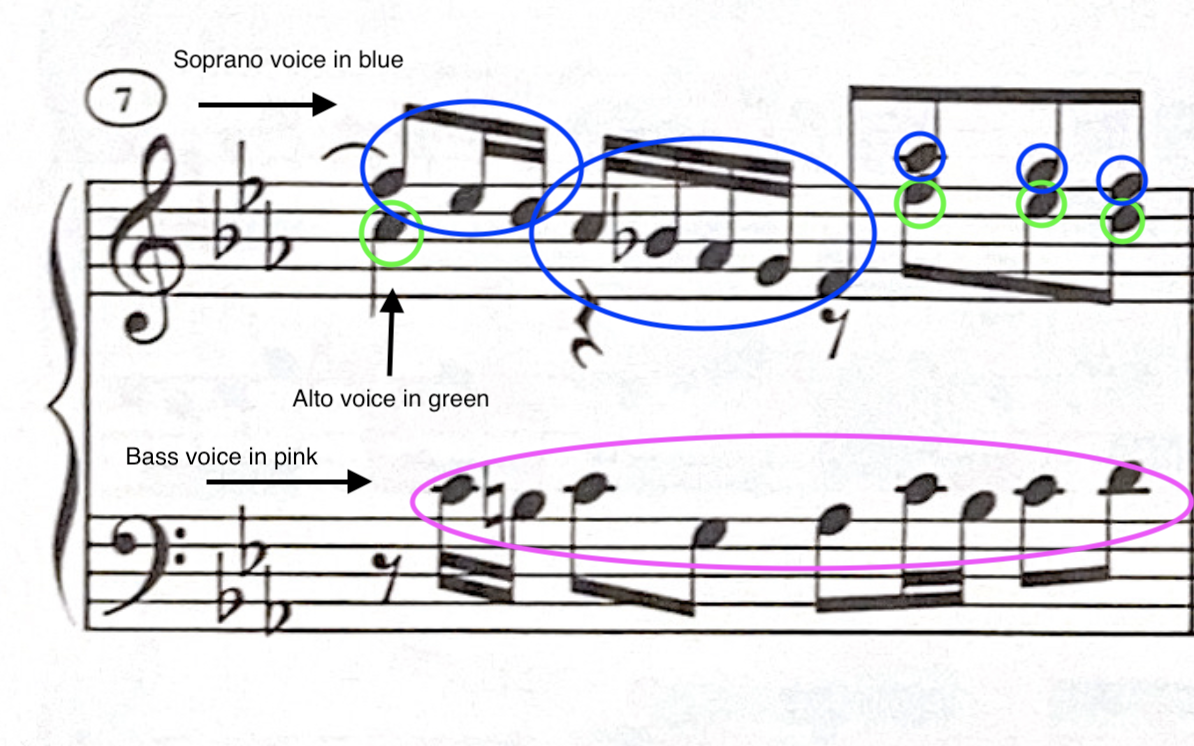
\includegraphics[width=.5\textwidth]{figures/fugue-three-voices.jpg}
    \caption{The three voices in Bach's \textit{Fugue in C Minor}}
    \label{fig:bach-fugue-three-voices}
\end{figure}
As seen in Figure \ref{fig:bach-fugue-three-voices}\autocite{Henle_2009}, there is a clear distinction between each voice. In the treble clef in the right-hand, the top line whose stems face upwards make up the soprano line (the line and notes circled in blue), and the bottom line with stems faced downwards make up the alto line (the line and notes circled in green). The bass clef will only contain the bass voice (the bottom line, circled in pink), as this fugue is only in three voices. It is a balanced piece, with structure and interactions between the three voices, soprano, alto, and bass--or subject, and two countersubjects. Structurally, the fugue starts with an exposition which marks the introduction of the subject line in the alto voice, as in Figure \ref{fig:bach-fugue-subject}\autocite{Henle_2009}. This subject is then seen in the soprano and bass voices, as in Figures \ref{fig:bach-fugue-subject}\autocite{Henle_2009} and circled in pink in Figure \ref{fig:bach-fugue-three-voices}\autocite{Henle_2009}. The soprano voice is circled in blue, and the bass voice in pink, showcasing the subject in both voices.
\begin{figure}
    \centering
    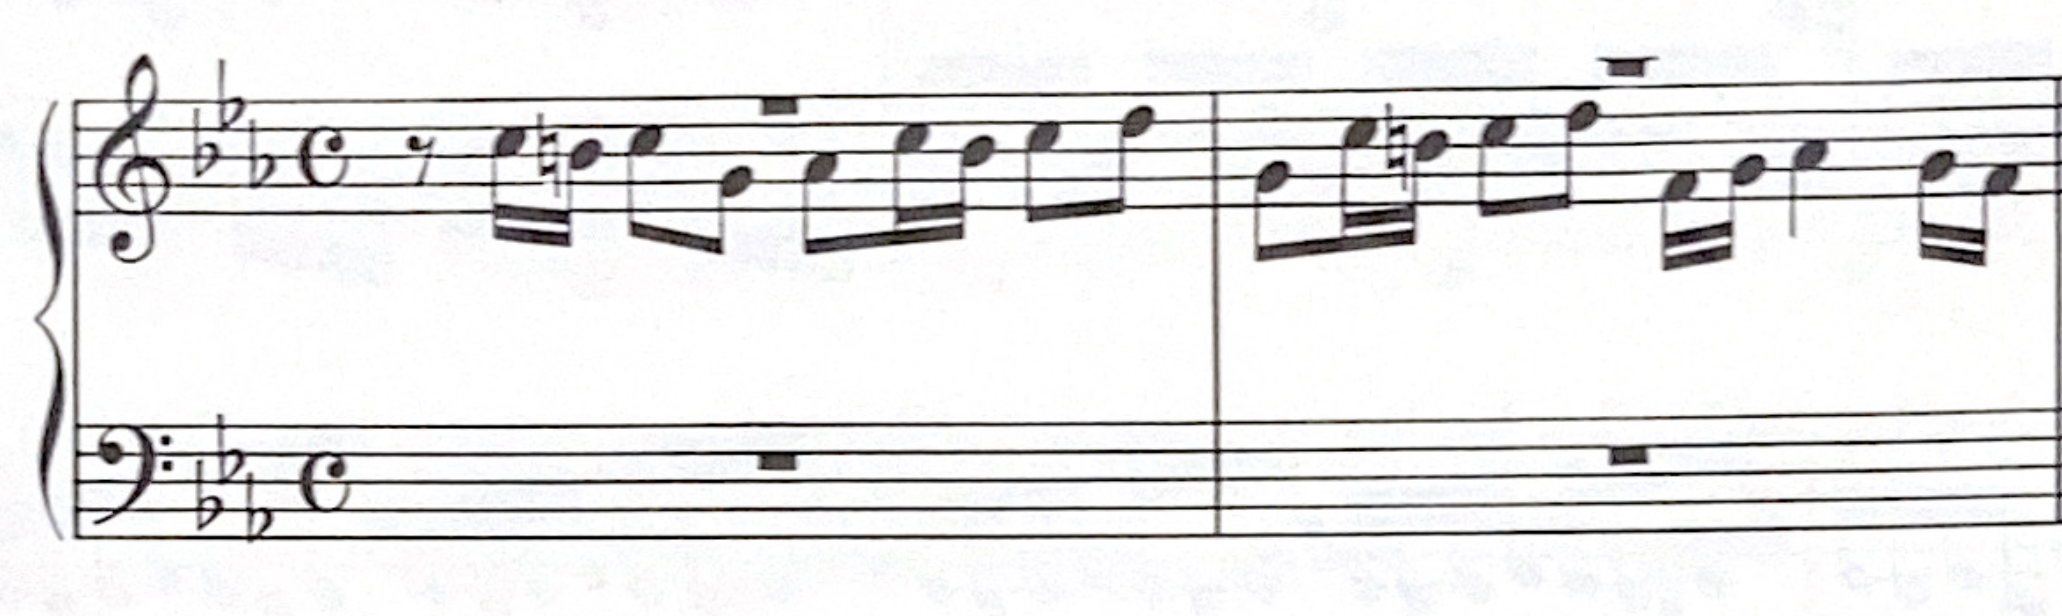
\includegraphics[width=\textwidth]{figures/bach-fugue-subject.jpg}
    \caption{The subject, in Bach's \textit{Fugue in C Minor}}
    \label{fig:bach-fugue-subject}
\end{figure}

The piece's third measure introduces the first countersubject in the alto voice, as in Figure \ref{fig:bach-fugue-first-countersubject}\autocite{Henle_2009}. Then, the second countersubject can be seen indicated rhythmically indicated in the second half of the first countersubject, before it is introduced on its own, as seen in Figure \ref{fig:bach-fugue-second-cs-indication}\autocite{Henle_2009}. The whole second countersubject then fully appears in the third and fourth beats of measure 7, circled in green, in Figure \ref{fig:bach-fugue-second-countersubject}\autocite{Henle_2009}.

\begin{figure}
    \centering
    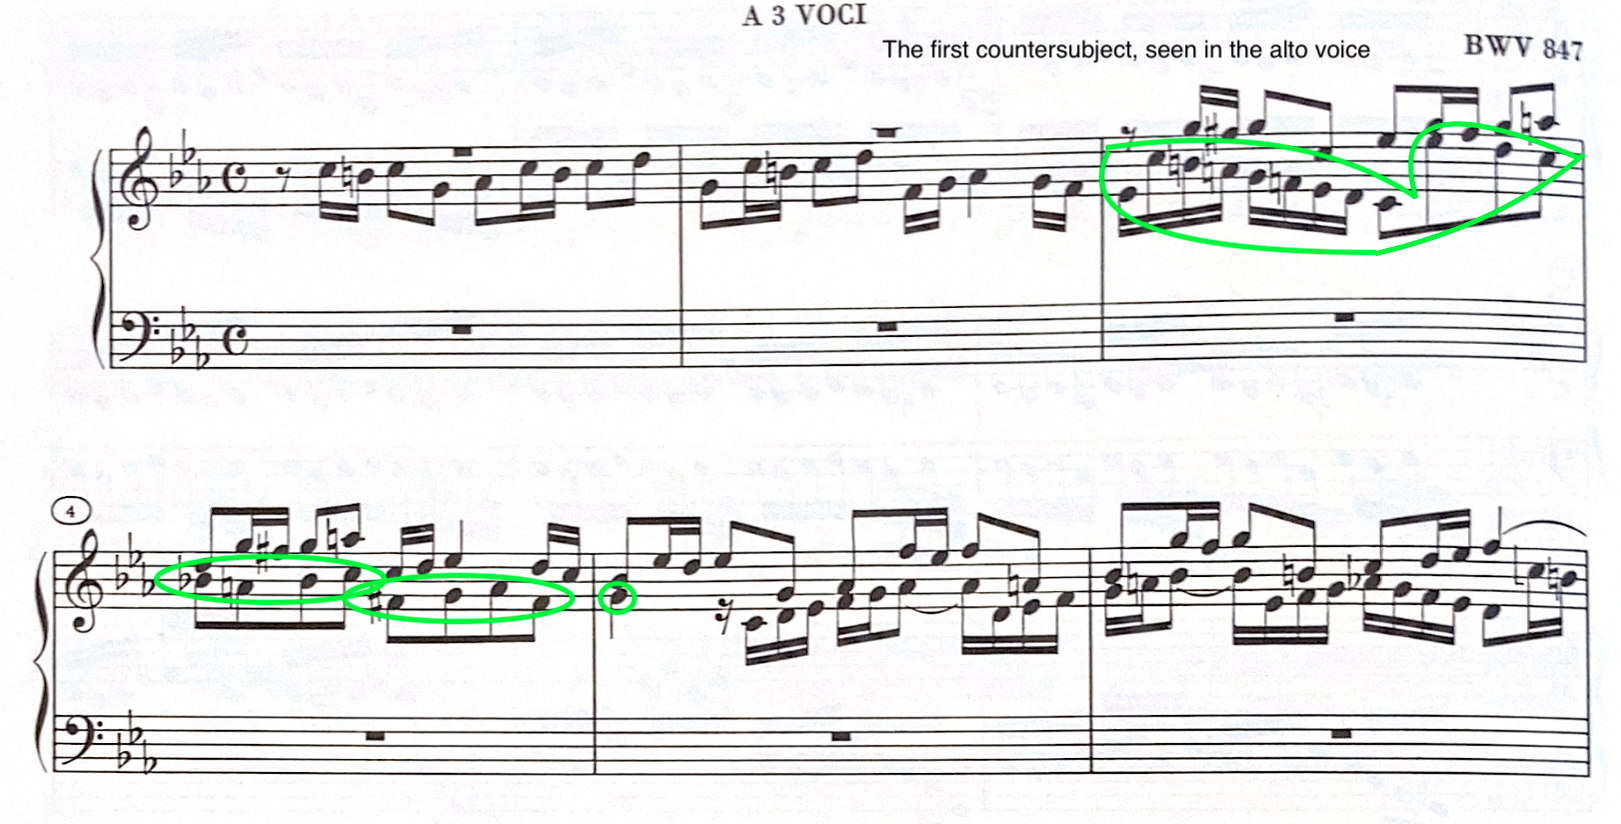
\includegraphics[width=\textwidth]{figures/bach-fugue-first-countersubject.jpg}
    \caption{The first countersubject, seen in the alto voice, in Bach's \textit{Fugue in C Minor}}
    \label{fig:bach-fugue-first-countersubject}
\end{figure}

\begin{figure}
    \centering
    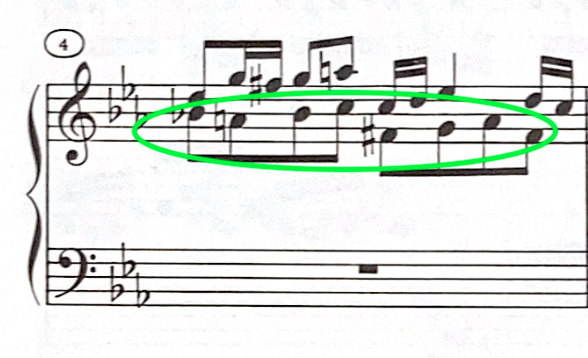
\includegraphics[width=0.5\textwidth]{figures/bach-fugue-second-cs-indication.jpg}
    \caption{The rhythmic indication of the second countersubject in Bach's \textit{Fugue in C Minor}, as circled in green, in the alto voice}
    \label{fig:bach-fugue-second-cs-indication}
\end{figure}

\begin{figure}
    \centering
    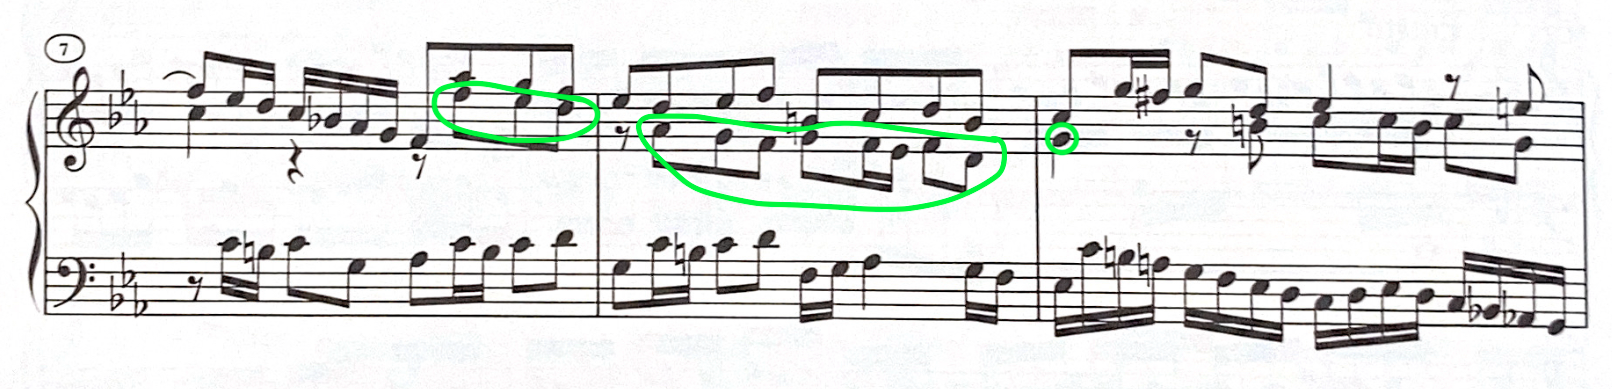
\includegraphics[width=\textwidth]{figures/bach-fugue-second-countersubject.jpg}
    \caption{The second countersubject, as found in the alto voice in its first appearance circled in green, from Bach's \textit{Fugue in C Minor}}
    \label{fig:bach-fugue-second-countersubject}
\end{figure}

Harmonically, the \textit{Fugue in C Minor} has a strong emphasis on minor keys, for dramatic effect. This is first seen in bar 3 of the \textit{Fugue in C Minor} in the top line, in Figure \ref{fig:bach-fugue-first-countersubject}\autocite{Henle_2009}, where the soprano voice modulates to the relative minor key, G harmonic minor. In the fugue's tension map\footnote{This is defined as a chart which details when there is tension in the music, and when the tension is resolved. Tension can be created through a chord's function, rhythm, or other methods.} there is more than a simple exposition\footnote{This is generally defined to be the section at the beginning of the piece, or near the beginning, in which one or more themes are presented according to a particular plan. These themes will be the basis of the rest of the movement or piece. In fugues specifically, the exposition is the opening section in which the voices enter one by one. Each voice states the principle theme (the subject), followed by the countersubject. All the voices after the fugue will wait to enter until the preceding voice has completed its statement of the subject.}\autocite{Walker_2001b}, subject entries, and coda\footnote{This is defined as the last part of a piece or melody, in which there is an implication that there is some addition being made to a standard form. In a fugue, this then refers to anything occurring after the last complete entry of the subject has been heard.}\autocite{Bullivant_2001}. 

\subsection{Three's a Crowd?}

Bach's fugue contains clear distinctions between the three voices; the right-hand plays two of the voices (soprano and alto), and the left-hand plays the remaining voice. My performance uses each of the three voices equally, when each voice contains a clear melody, or counter melody. This will usually lead to the soprano and alto voices being heard most often, although the bass voice will occasionally play the subject or a countermelody. In Figure \ref{fig:bach-fugue-subject}\autocite{Henle_2009}, the first time the subject is heard is in the soprano voice, as it plays a combination of sixteenth notes and eighth notes. The alto voice then introduces the first countersubject in measure 3 (Figure \ref{fig:bach-fugue-first-countersubject}\autocite{Henle_2009}), and it is this subject and countersubject, along with its variations, which I emphasize, and player slightly louder than the material other voices sound. So, in instances in which all three voices sound at the same time, but only two voices contain a subject or countersubject, I perform the phrase in a balance which prioritizes the subject and countersubject. As in Figure \ref{fig:bach-fugue-second-countersubject}\autocite{Henle_2009}, here the alto voice sounds the second countersubject of the piece, which the bass voice contains the subject. The soprano voice only contains harmony to both the subject and countersubject, so therefore will not be played as loudly as the other two voices. 

It is in phrases such as these in which I am aware of the need for the separation between voices. When I play, each voice should be distinguishable from each of the other voices, without much effort from the listener. Each voice plays its own role in the piece, and I perform as if each voice contains an entirely separate melody, even if the voice contains a harmony instead of a countersubject. 

